\documentclass[och, master]{SCWorks}

\usepackage[utf8]{inputenc}
\usepackage[T2A]{fontenc}
\usepackage[russian]{babel}

\usepackage{pdfpages}

\usepackage{hyperref}
\usepackage{amsfonts}
\usepackage{commath}
\usepackage{amsthm}
\usepackage{amssymb}
\usepackage{float}

\theoremstyle{plain}
\newtheorem{thethm}{Теорема}

\theoremstyle{plain}
\newtheorem{lemma}{Лемма}

\theoremstyle{plain}
\newtheorem{note}{Замечание}

\theoremstyle{definition}
\newtheorem{defn}{Определение} 

\newtheorem{exmp}{Пример}

\geometry{verbose,a4paper,tmargin=2cm,bmargin=2cm,lmargin=2.5cm,rmargin=1.5cm}

\hypersetup{
    colorlinks=true, %set true if you want colored links
    linktoc=all,     %set to all if you want both sect. and subsect. linked
    linkcolor=blue,  %choose some color if you want links to stand out
}

\author{Sharov Alex}

\begin{document}

%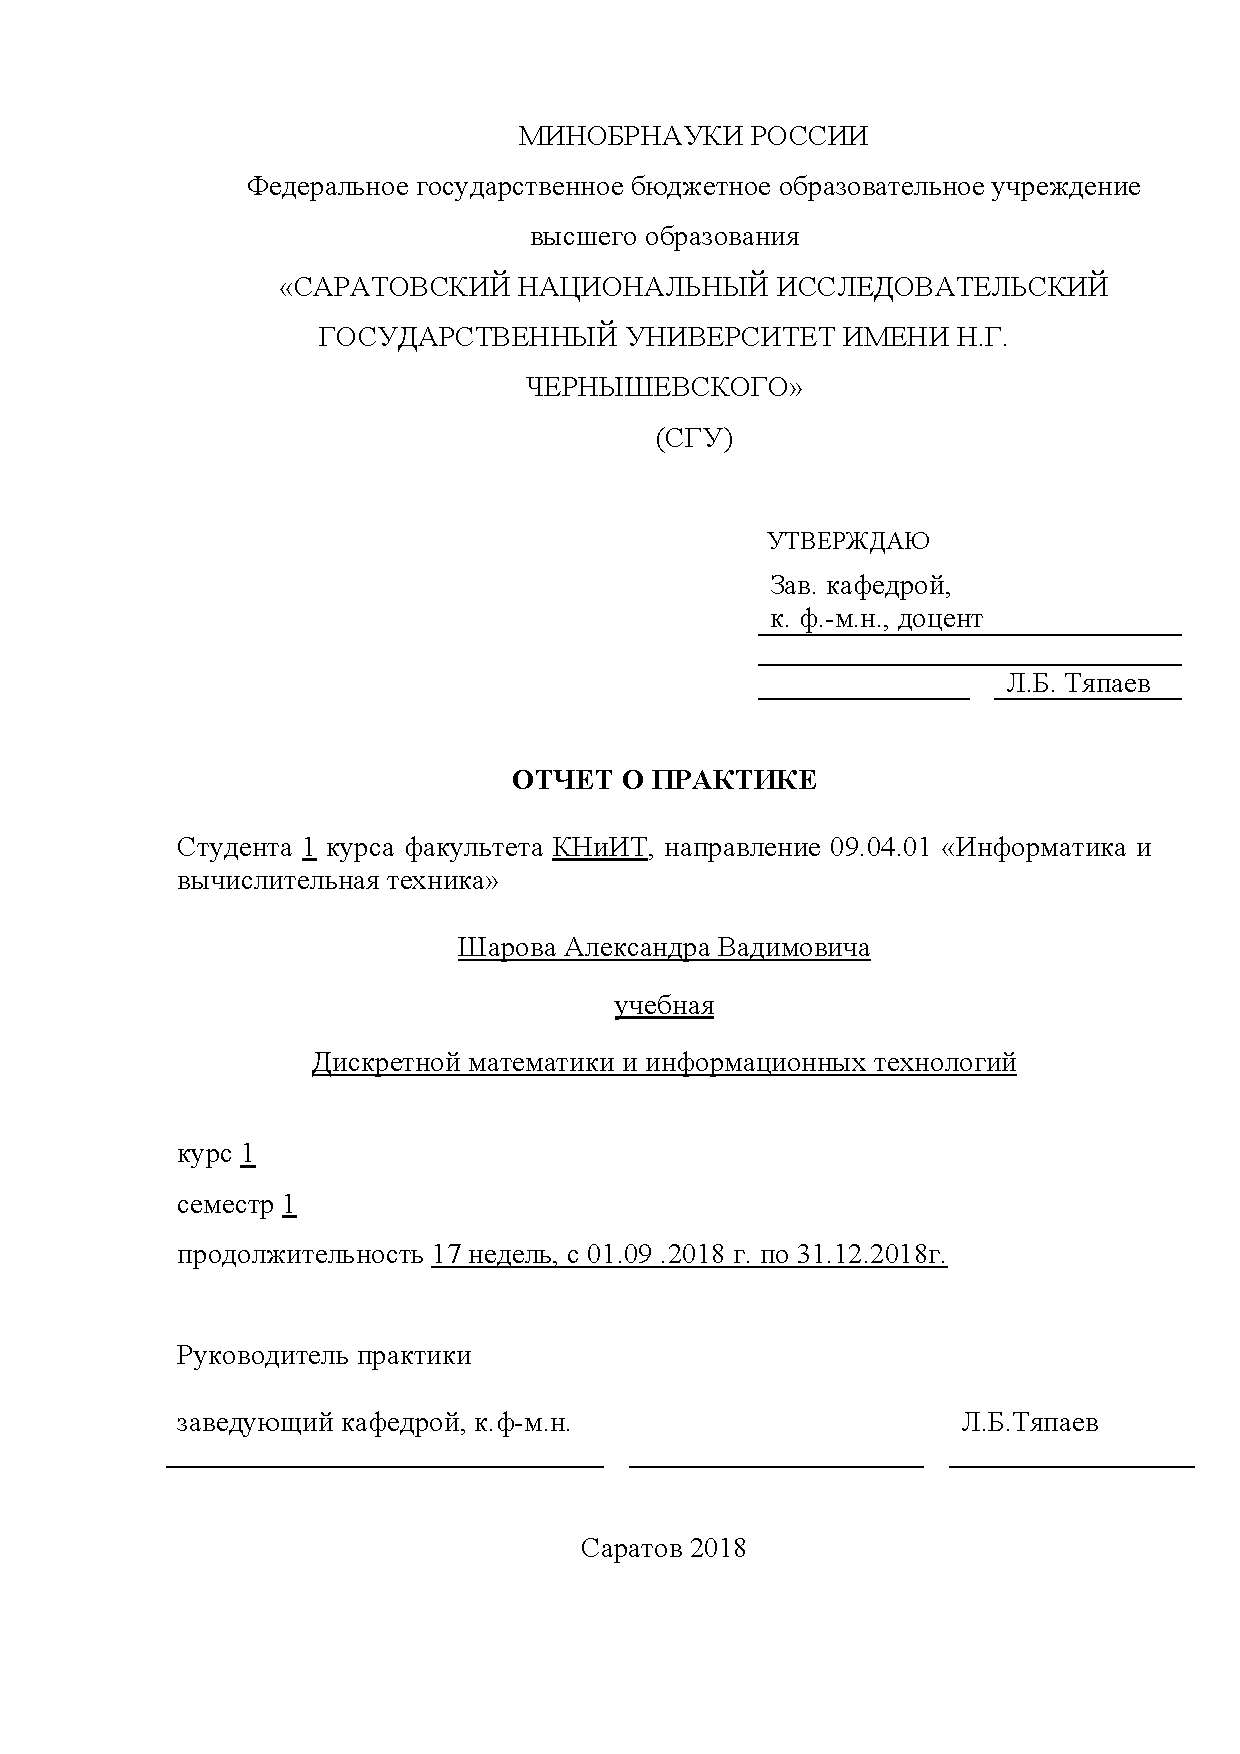
\includepdf[pages={1}]{titul.pdf}
\setcounter{tocdepth}{2}

\tableofcontents

\definitions

\begin{enumerate}
	\item $\mathbb {Z}$ -- кольцо целых рациональных чисел
	\item $\mathbb {Z}_{+}$ -- множество натуральных чисел $\mathbb {N}$
	\item ${N}_0=\{0,1,\dots\}$
	\item $\mathbb {P}$ -- множество простых чисел
	\item Сепарабельное пространство -- топологическое пространство, в котором можно выделить счётное всюду плотное подмножество
	\item Плотное множество -- подмножество пространства, точками которого можно сколь угодно хорошо приблизить любую точку объемлющего пространства.
	\item Счётное множество -- бесконечное множество, элементы которого возможно пронумеровать натуральными числами.
	\item Хаусдорфово пространство — топологическое пространство, удовлетворяющее сильной аксиоме отделимости $T_2$.
	\item Множество из $\mathbb {R}^n$ называется компактом, если из любой последовательности его точек можно выделить сходящуюся подпоследовательность, предел которой принадлежит этому множеству.
	\item Локально компактное пространство — топологическое пространство, у каждой точки которого существует открытая окрестность, замыкание которой компактно.
	\item Размерностью полного метрического пространства $X$ называется наименьшее целое число $n$ такое, что для любого покрытия пространства $X$ существуют вписанное в него подпокрытие кратности $n+1$.
	\item Конечный автомат — абстрактный автомат, число возможных внутренних состояний которого конечно.
	\item Абстрактный автомат с выделенным начальным состоянием называется инициальным автоматом. \cite{bib:automata:elements}
	\item Автомат Мили конечный автомат, выходная последовательность которого зависит от состояния автомата и входных сигналов. Это означает, что в графе состояний каждому ребру соответствует некоторое значение (выходной символ). В вершины графа автомата записываются выходящие сигналы, а дугам графа приписывают условие перехода из одного состояния в другое, а также входящие сигналы. \cite{bib:automata:elements}
	\item Автомат Мура (абстрактный автомат второго рода) - конечный автомат, выходное значение сигнала в котором зависит лишь от текущего состояния данного автомата, и не зависит напрямую, в отличие от автомата Мили, от входных значений. \cite{bib:automata:elements}
	
\end{enumerate}

\intro
Со времен Ньютона и Лейбница вещественные числа применялись как основной математический объект, который казалось бы отлично подходил для описания окружающего мира. В большинстве практических задач обычно составлялись уравнения и в последствии искалось числовое решение над полем действительных чисел $\mathbb {R}$. Обоснования почему в качестве описательного элемента выбрали именно поле $\mathbb {R}$ даже не стоял. В качестве пространства стандартом де-факто долгое время являлось пространство $\mathbb {R}^3$, а уже после открытий Римана и Эйнштейна $\mathbb {R}^4$. 

С течением времени и наращиванием математического аппарата представление о том, что пространство $\mathbb {R}^3$ является наиболее подходящим для описания реального мира все усиливалось, но надо понимать, что евклидово пространство $\mathbb {R}^3$ не более чем удачно выбранная модель описания реального физического пространства. 

Так как реальный мир построен на евклидовой геометрии, то получается, что и она очень хорошо описывается вещественными числами, но в случае если бы мы могли отказаться от использования данной геометрии для изучения реального мира мы бы могли отказаться и от вещественной числовой системы. Но какую выбрать систему в данном случае? На этот ответ лучше всего отвечает теория $p$-адического исчисления, которая является с математической точки зрения более подходящей для описания тех объектов, с которыми приходиться работать в задачах физики, биологии и криптографии.\cite{bib:kozirev:2008}

Целью данной курсовой работы является построение $p$-адического автомата для функции $f: \mathbb Z_p \rightarrow \mathbb Z_p$ вида $f(x)=cx$, где $c=\frac{n}{m}, n,m \in \mathbb Z$. В первых двух разделах будет приведен обзор на инструменты $p$-адического анализа, а в третьем разделе будет описана основная теорема\cite{bib:crypto:anashin} для детерминированных функций и непосредственно пошаговое построение автомата для функции $f(x)=cx$.

\section{p-Адические числа}

\subsection{p-Адическая норма}

\begin{defn}
Пусть $M$ - некоторое непустое множество, и пусть \linebreak ${d: M \times M \rightarrow \mathbb {R}_{\ge0}}$ -- функция двух переменных, определенная на этом множестве и принимающая значения во множестве действительных неотрицательных чисел. Функция $d$ называется метрикой (а множество $M$ -- метрическим пространством), если $d$ удоволетворяет трем условиям:

\begin{enumerate} 
	\item Для каждой пары $a, b \in M$ справедливо: $d(a, b)=0$ тогда и только тогда, когда $a=b$.
	\item Для каждой пары $a, b \in M$ справедливо равенство $d(a, b) = d(b, a)$.
	\item Для каждой тройки $a, b, c \in M$ справедливо неравенство $d(a, b) \le d(a, c) + d(c, b)$.
\end{enumerate}
\end{defn}

\begin{exmp}
Множество $\mathbb {R}$ всех действительных чисел есть метрическое пространство с метрикой $d(a, b)= \abs{a-b}$, где $\abs{.}$ есть абсолютная величина.
\end{exmp}


\begin{defn}
Функция $\norm{.}$, определенная на произвольном коммутативном кольце R и принимающая значения в $\mathbb {R}_{\ge 0}$ называется нормой (также, абсолютной величиной), если она удовлетворяет следующим условиям:

\begin{enumerate} 
	\item Для любого $a \in R$ справедливо, что $\norm{a}=0$ тогда и только тогда, когда $a=0$.
	\item Для каждой пары $a, b \in R$ справедливо равенство $\norm{a \cdot b} = \norm{a} \cdot \norm{b}$.
	\item Для каждой пары $a, b \in R$ справедливо неравенство треугольника: $\norm{a + b} \le \norm{a} + \norm{b}$
\end{enumerate}
\end{defn}

Из определения следует, что если положить $d(a, b)= \norm{a - b}$, то фактически будет задана метрика $d$ на кольце $R$. Данная метрика называется метрикой, индуцированной нормой $\norm{.}$.

\begin{defn}
Пусть $p \in \mathbb {P}$ -- некоторое простое число. В поле $\mathbb {Q}$ введем другую норму $\norm{.}_p$ по правилу:

\begin{enumerate} 
	\item $\norm{0}_p = 0$,
	\item $\norm{n}_p = p ^ {-ord_pn}$,
\end{enumerate}

\noindent где $n > 0$ некоторое натуральное число, а $ord_pn$ показатель степени, в которой число $p$ входит в это произведение. В этом случае норма $\norm{.}_p$ называется $p$-адической нормой.
\end{defn}

Норма $\norm{.}_p$  удовлетворяет всеми характерными свойствами нормы даже в более сильной форме, а именно:

\begin{enumerate} 
	\item $\norm{x}_p \ge 0$, причем $\norm{x}_p = 0$ если $x = 0$.
	\item $\norm{xy}_p = \norm{x}_p \cdot \norm{y}_p$.
	\item $\norm{x + y}_p \le \max(\norm{x}_p, \norm{y}_p)$ \cite{bib:analysis:volovich}
\end{enumerate}

Заметим, что норма $\norm{x}_p$ может принимать лишь счетное число значений $p ^ {-ord_pn}$.

Также, норма $\norm{x}_p$ определяет ультраметрику на $\mathbb {Q}$. Данная норма неархимедова, так как $\norm{nx}_p \le \norm{x}_p \forall n \in \mathbb {Q}_{+}$.

\begin{thethm}
	Нормы $\norm{.}$ и $\norm{.}_p$ $\forall p = 2, 3, \dots$ исчерпывают все нетривиальные неэквивалентные нормы поля рациональных чисел $\mathbb {Q}$.
\end{thethm}


\subsection{p-Адические числа}

\begin{defn}
Пополнение поля $\mathbb {Q}$ по $p$-адической норме образует поле $\mathbb {Q}_p$ $p$-адических чисел. Поле $\mathbb {Q}_p$ аналогично полю $\mathbb {R} = \mathbb {Q}_{\infty}$ вещественных чисел, получаемых пополнение поля $\mathbb {Q}$ по норме $\norm{x}=\norm{x}_{\infty}$.
\end{defn}


\begin{defn}
Любое $p$-адическое число $x \ne 0$ однозначно представляется в каноническом виде

\begin{equation} \label{numbers:decomposition}
	x = p^{\gamma} \cdot (x_0 + x_1\cdot p + x_2 \cdot p^2 + \dots
\end{equation}

\noindent где $\gamma = \gamma(x) \in \mathbb {Z}$ и $x_j$ -- целые числа такие, что $0 \le x_j \le p-1$, $x_0 > 0,$ \linebreak $(j=0,1,\dots)$. 
\end{defn}

Представление \eqref{numbers:decomposition} аналогично разложению любого вещественного числа $x$ в бесконечную десятичную дробь:
\begin{equation*}
\begin{aligned}
	x=\pm10^\gamma \cdot (x_0 + x_1 \cdot 10^{-1} + x_2 \cdot 10^{-2} + \dots),\\
	\gamma \in \mathbb {Z}, x_j = 0, 1, \dots, 9, x_0 > 0,
\end{aligned}
\end{equation*}

\noindent и доказывается аналогично.

Помимо разложения, представление \eqref{numbers:decomposition} дает рациональные числа тогда и только тогда, когда, начиная с некоторого номера числа $x_j, j=0,1,\dots$ образуют периодическую последовательность.

\begin{defn}
Поле $\mathbb {Q}_p$ является коммутативно-ассоциативной группой по сложению;
\end{defn}

\begin{defn}
Поле $\mathbb {Q}_p^*=\mathbb {Q}_p \setminus \{0\}$ является коммутативно-ассоциативной группой по умножению;
\end{defn}

\begin{defn}
Поле $\mathbb {Q}_p^*$ называется мультипликативной группой поля $\mathbb {Q}_p$\cite{bib:analysis:baker};
\end{defn}

\begin{defn}
$p$-адические числа $x$, для которых $\norm{x}_p \le 1$ (т.e. $\gamma(x) \ge 0$ или $\{x\}_p=0$), называются целыми $p$-адическими числами, и их множество обозначается $\mathbb {Z}_p$. Множество $\mathbb {Z}_p$ является подкольцом кольца $\mathbb {Q}_p$; $\mathbb {Z}_+$ плотно в $\mathbb {Z}_p$. Целые числа $x \in \mathbb {Z}_p$, для которых $\norm{x}_p=1$, называютсяются единицами в $\mathbb {Z}_p$. \cite{bib:analysis:vladimirov}
\end{defn}

Совокупность элементов $x$ из $\mathbb {Z}_p$, для которых $\norm{x}_p < 1$ (т.e. $\gamma(x) \ge 0$ или $\norm{x}_p \le \frac{1}{p}$) образуют главный идеал кольца $\mathbb {Z}_p$; Данный идеал имеет вид $p\mathbb {Z}_p$. Поле вычетов $\mathbb {Z}_p \setminus p\mathbb {Z}_p$ состоит из $p$ элементов. В мультипликативной группе поля $\mathbb {Z}_p \setminus p\mathbb {Z}_p$ существует единица $\eta \ne 1$ порядка $p-1$ такая, что элементы $0, \eta, \eta^2, \dots, \eta^{p-1} = 1$ образуют полный набор представителей классов вычетов поля $\mathbb {Z}_p \setminus p\mathbb {Z}_p$.

\subsection{Пространство p-адических чисел $\mathbb {Q}_p$}
В силу свойств $p$-адической нормы норма в поле $\mathbb {Q}_p$ удовлетворяет неравенству треугольника:
$$\norm{x + y}_p \le \max(\norm{x}_p, \norm{y}_p) \le \norm{x}_p + \norm{y}_p, x,y \in \mathbb {Q}_p.$$
\noindent Следовательно в $\mathbb {Q}_p$ можно ввести метрику:

\begin{equation}
	\rho (x,y)=\norm{x-y}_p.
\end{equation}

\noindent При этом $\mathbb {Q}_p$ становится полным метрическим пространством. Из представления \eqref{numbers:decomposition} следует сепарабельность $\mathbb {Q}_p$.  

\begin{defn}
$B_{\gamma}(a)$ -- круг радиуса $p^{\gamma^p}$ с центром в точке $a \in \mathbb {Q}_p$:
\begin{equation}
	B_\gamma(a) = \bigg\{x: \norm{x-a}_p \le p^{\gamma} \bigg\}, \gamma \in \mathbb {Z}
\end{equation}
\end{defn}

\begin{defn}
$S_{\gamma}(a)$ -- граница радиуса $p^{\gamma^p}$.
\begin{equation}
	S_\gamma(a) = \bigg\{x: \norm{x-a}_p = p^{\gamma} \bigg\}, \gamma \in \mathbb {Z}
\end{equation}
\end{defn}

\begin{lemma}
Если $b \in B_{\gamma}(a)$, то $B_{\gamma}(b)=B_{\gamma}(a)$.
\end{lemma}

\begin{note}
Круг $B_{\gamma}(a)$ и окружность $S_{\gamma}(a)$ -- открыто-замкнутые множества в $\mathbb {Q}_p$.
\end{note}

\begin{note}
Всякая точка круга $B_{\gamma}(a)$ является его центром.
\end{note}

\begin{note}
Любые два круга в $\mathbb {Q}_p$ либо не имеют общих точек, либо один содержится в другом.
\end{note}

\begin{note}
Всякое открытое множество в $\mathbb {Q}_p$ есть объединение не более чем счетного числа кругов без общих точек.
\end{note}

\begin{lemma} \label{lemma:2}
Если множество $M \subset \mathbb {Q}_p$ содержит две различные точки $a$ и $b$, $a \ne b$, то его можно представить в виде объединения непересекающихся открыто-замкнутых (в $M$) множеств $M_1, M_2$ таких, что $a \in M_1, b \in M_2$.
\end{lemma}

Лемма \eqref{lemma:2} утверждает, что всякое множество пространства $\mathbb {Q}_p$, состоящее из более чем одной точки, несвязно. Другими словами, связная компонента любой точки совпадает с самой точкой. Из этого следует, что $\mathbb {Q}_p$ является вполне несвязным пространством.

Если рассматривать лемму для случая, когда множество $M$ состоит только из двух точек $a$ и $b$, убеждаемся, что существует непересекающиеся окрестности этих точек. Из этого можно сделать вывод, что пространство $\mathbb {Q}_p$ хаусдорфово.

\begin{lemma}
Для того чтобы множество $K \subset \mathbb {Q}_p$ было компактом, необходимо и достаточно, чтобы оно было замкнутым и ограниченным в $\mathbb {Q}_p$
\end{lemma}

\begin{note}
Всякий круг $B_{\gamma}(a)$ является и окружность $S_{\gamma}(a)$ компакты.
\end{note}

\begin{note}
Пространство $\mathbb {Q}_p$ локально компактное.
\end{note}

\begin{note}
Всякий компакт можно покрыть конечным числом кругов фиксированного радиуса без общих точек.
\end{note}

\begin{note}
В пространстве $\mathbb {Q}_p$ справедлива лемма Гейне-Бореля: из каждого бесконечного покрытия компакта $K$ можно выбрать конечное покрытие $K$.
\end{note}

\begin{thethm}
Размерность пространства $\mathbb {Q}_p$ равна $0$.
\end{thethm}

\section{p-Адический анализ в $\mathbb {Z}_p$}

Так как компакт $\mathbb {Z}_p$ есть пополнение множества $\mathbb {N}_0$ по метрике \linebreak ${d_p(x,y)=\norm{x-y}_p}$, то любое число из $\mathbb {Z}_p$ есть предел последовательности чисел из $\mathbb {N}_0$.

\begin{defn}
$p$-адическое целое $z$ является пределом последовательности $\{z_i\}^{\infty}_{i=0}$, если если для любого $\epsilon > 0$ найдется $N$ такое, что $\norm{z_i-z}_p < \epsilon$ как только $i>N$. \cite{bib:analysis:anashin}
\end{defn}

\begin{defn}
$p$-адическое целое $z$ есть предел последовательности $\{z_i\}^{\infty}_{i=0}$, если для любого (достаточно большого) положительного рационального целого $K$ найдется $N$ такое, что ${z_i \equiv z \pmod p^K}$ при всех $i>N$. \cite{bib:analysis:anashin}
\end{defn}

\begin{note}
По определению $p$-адической метрики $\norm{z_i-z}_p \le p^{-K}$ тогда и только тогда, когда $z_i \equiv z \pmod p^K$. \cite{bib:analysis:anashin}
\end{note}

\begin{defn}
Функция $f:\mathbb {Z}_p \rightarrow \mathbb {Z}_p$ называется непрерывной в точке $z \in \mathbb {Z}_p$, если для любого (достаточно большого) положительного рационального целого $M$ найдется положительное рациональное целое $L$ такое, что ${f(x) \equiv f(z) \pmod p^M}$ как только $x \equiv z \pmod{p^L}$. \cite{bib:analysis:anashin}
\end{defn}

\begin{defn}
Функция $f$ называется равномерно непрерывной на $\mathbb {Z}_p$, если $f$ непрерывна в каждой точке $z \in \mathbb {Z}_p$, и $L$ зависит только от $M$ и не зависит от $z$.\cite{bib:analysis:ciocan}
\end{defn}


\subsection{$p$-адическая дифференцируемость}

\begin{defn}
Функция $f:\mathbb {Z}_p \rightarrow \mathbb {Z}_p$ называется дифференцируемой в точке $z \in \mathbb {Z}_p$, если существует $p$-адическое число $f'(x) \in \mathbb {Q}_p$ такое, что для любого $M \in \mathbb {N}$ справедливо
\begin{equation} \label{derivative:1}
	\norm{\frac{f(x+h)-f(x)}{h} - f'(x)}_p \le \frac{1}{p^M},
\end{equation}

\noindent если $h$ достаточно мало, т.e. когда $\norm{h}_p \le p^{-K}$, где $K=K(M)$ достаточно велико.
\end{defn}

\begin{defn}
Функция $f$ называется равномерно дифференцируемой (на $\mathbb {Z}_p$), если неравенство \eqref{derivative:1} выполняется одновременно для всех $x \in \mathbb {Z}_p$ как только $h$ достаточно мало. \cite{bib:analysis:anashin:en}
\end{defn}

\begin{lemma}
Если совместимая функция $f:\mathbb {Z}_p \rightarrow \mathbb {Z}_p$ дифференцируема в точке $x \in \mathbb {Z}_p$, то $f'(x) \in \mathbb {Z}_p$.
\end{lemma}

\begin{defn}
Функция $f:\mathbb {Z}_p \rightarrow \mathbb {Z}_p$ называется дифференцируемой в точке $x \in \mathbb {Z}_p$, если существует $p$-адическое число $f'(x) \in \mathbb {Q}_p$ такое, что для любого $M \in \mathbb {N}$ справедливо
\begin{equation} \label{derivative:2}
	f(x+h) \equiv f(x) + h \cdot f'(x) \pmod p^{M + ord_p h}
\end{equation}
\end{defn}

\begin{defn}
Функция $f$ называется равномерно дифференцируемой (на $\mathbb {Z}_p$), если неравенство \eqref{derivative:2} выполняется одновременно для всех $x \in \mathbb {Z}_p$ как только $h$ достаточно мало, т.e. когда $ord_p h \ge K=K(M)$ для достаточно большого $K \in \mathbb {N}$.
\end{defn}

\begin{note}
Правила дифференцирования не зависят от метрики: для вычисления производных суммы, частного и сложной функции в $p$-адическом анализе используются те же формулы, что и в действительном.
\end{note}

\begin{note}
Между действительным и $p$-адическим анализом существует резкое различие например в том, что в и в том, и в в другом случае производная константы равна $0$, однако в $p$-адическом анализе в отличии от действительного равенство нулю производной некоторой функции не означает, что эта функция константа.
\end{note}

\section{p-Адические автоматы}

В данном разделе мы будем заниматься построением автомата для функции вида $f(x)=cx$, где $c=\frac{n}{m}, n,m \in \mathbb Z$. Перед тем как рассматривать построение автомата, рассмотрим основные определения \cite{bib:automata:phd} и основную теорему, которая говорит о том, что для каждой совместимой функции $f: \mathbb {Z}_p \rightarrow \mathbb {Z}_p$ можно построить соответствующий ей автомат.

Зафиксируем простое число $p$. Если рассматривать стандартный алгоритм сложения столбиком двух многоразрядных чисел в $p$-адической системе счисления, то видно, что эта операция может быть реализована с помощью конечного автомата Мили $\Sigma_p$, называемого последовательным сумматором, у которого два $p$-ичных входа и один $p$-ичный выход.


\begin{figure}[H]
\centerline{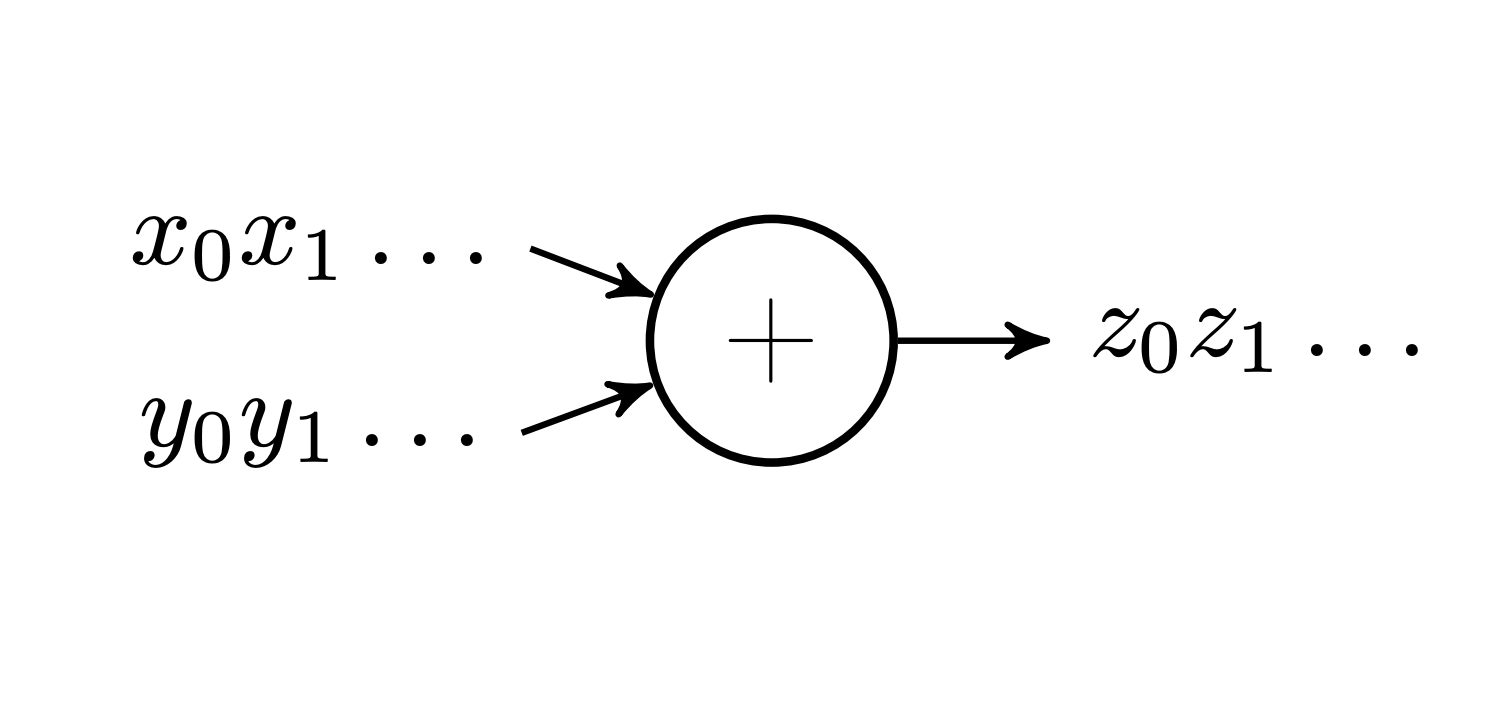
\includegraphics[width=0.5\linewidth]{img/automata_1}}
\caption{Автомат $\Sigma_p$}
\label{img:automata:1}
\end{figure}

\begin{figure}[H]
\centerline{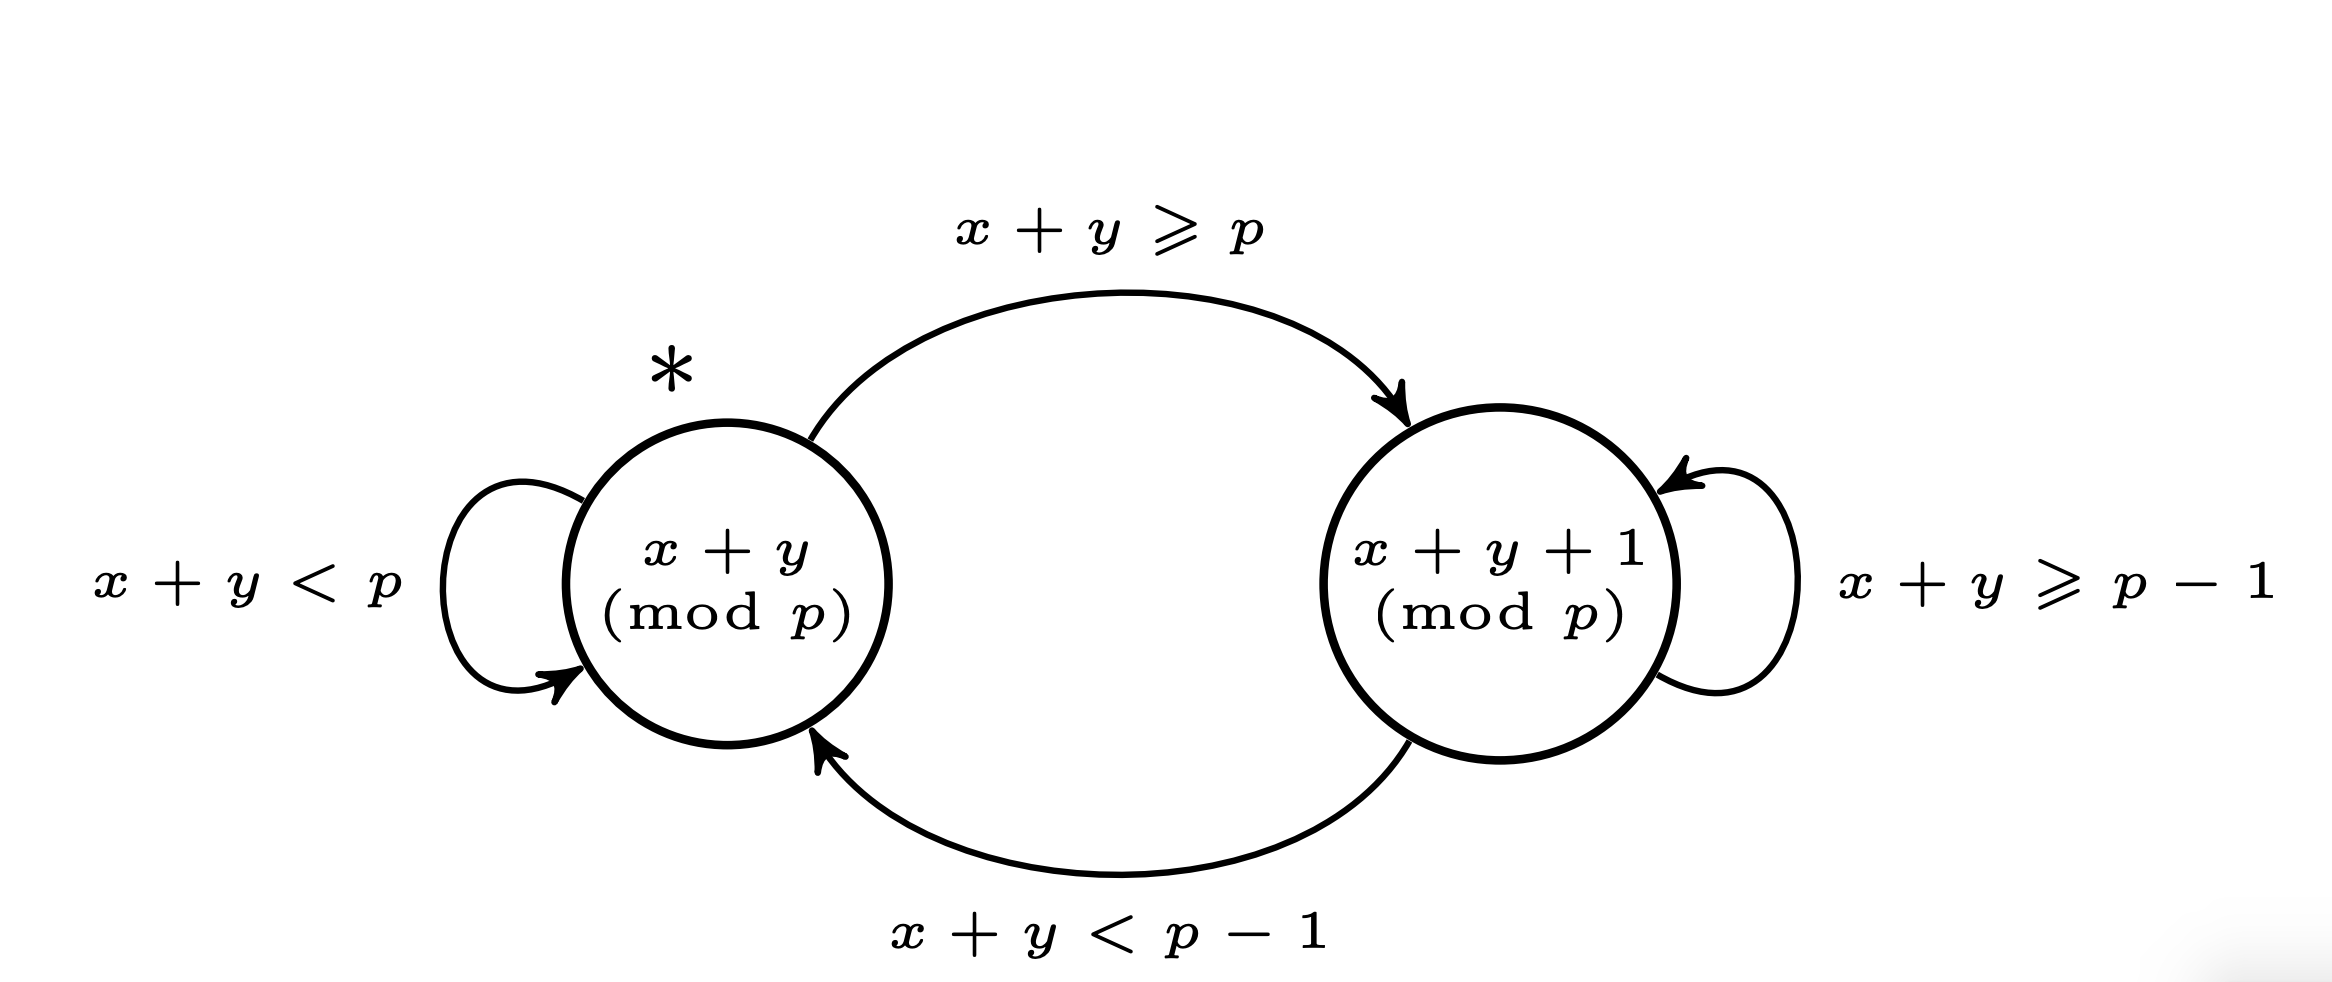
\includegraphics[width=0.5\linewidth]{img/automata_2}}
\caption{Диаграмма переходов автомата $\Sigma_p$}
\label{img:automata:2}
\end{figure}


\noindentКак видно из диаграммы переходов автомата $\Sigma_p$ на рис. \ref{img:automata:2}, у автомата два состояния, соответствующие наличию и отсутствию переноса на данный момент вычисления, а  его состоянием является состояние с отсутствием переноса. Внутри каждого состояния указана соответствующая функция выхода, а на стрелках - условия при которых происходит данный переход. 

Автомат $\Sigma_p$ реализует ограниченно-детерминированную функцию $\Sigma_p(x,y)$, которую можно отождествить со сложением $x+y$ в кольце $\mathbb Z_p$, если рассматривать сверхслова $x_0x_1\cdots$ над алфавитом $E_p=\{0,1,\cdots, p-1\}$ как элементы $\sum_{i \ge 0} x_ip^i$ кольца $\mathbb Z_p$. Такое отождествление позволяет рассматривать любую детерминированную функцию $f(x_1,\cdots, x_n)$, определенную и принимающую свои значения на множестве сверхслов над алфавитом $E_p$, как функцию $f: \mathbb {Z}^{n}_{p} \rightarrow \mathbb {Z}_p$.


Такая интерпретация детерминированных функций рассматривалась Лунцем в его работе \cite{bib:automata:lunz}, где такие функции назывались $p$-адическими автоматами. При этом выделяется класс $p$-адических автоматов, являющихся линейными однородными функциями вида:

$$ f(x_1, \cdots, x_n) = c_1x_1 + c_2x_2 + \cdots + c_n x_n,$$

\noindent где $c_1, \cdots, c_n \in Q \cap \mathbb Z_p$, и показано, что это в точности все линейные однородные функции, реализуемые конечными автоматами. Отметим также, что $p$-адическая интерпретация детерминированных функций позволяет изучать их свойства, привлекая
аппарат теории динамических систем \cite{bib:dynamics:anashin} и p-адического анализа \cite{bib:analisys:anashin}.

Рассмотрим автоматы реализующие функцию вида $f(x)=cx$, где $c \in Q \cap \mathbb Z_p$. Множество таких автоматов образует кольцо $Z_{(p)}$ относительно операции сложения, определенной с помощью автомата $\Sigma_p$ (рис. \ref{img:automata:3}), и операции умножения, определенной как суперпозиция двух автоматов (рис.\ref{img:automata:4}). 

\begin{figure}[H]
\centerline{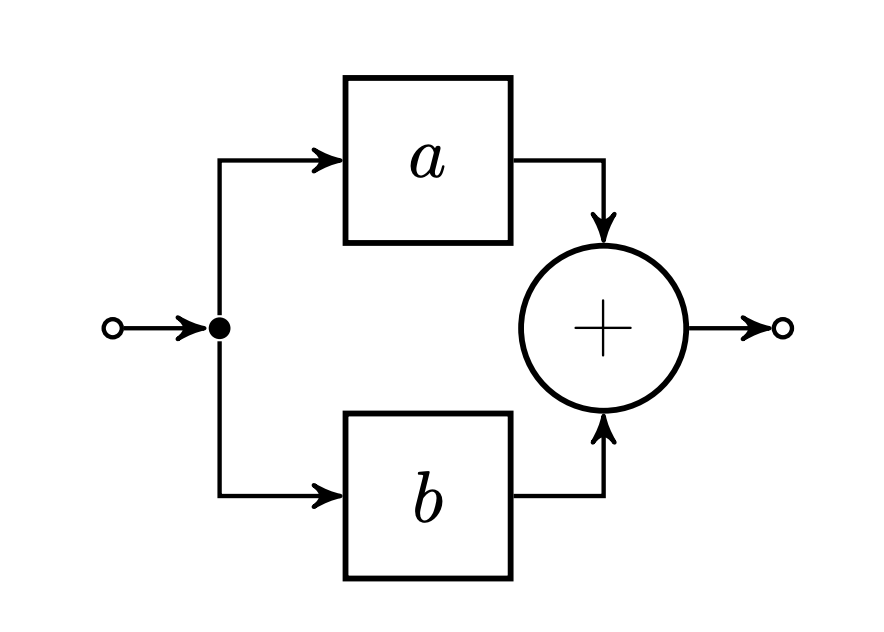
\includegraphics[width=0.5\linewidth]{img/automata_3}}
\caption{Сложение автоматов $ax$ и $bx$}
\label{img:automata:3}
\end{figure}

\begin{figure}[H]
\centerline{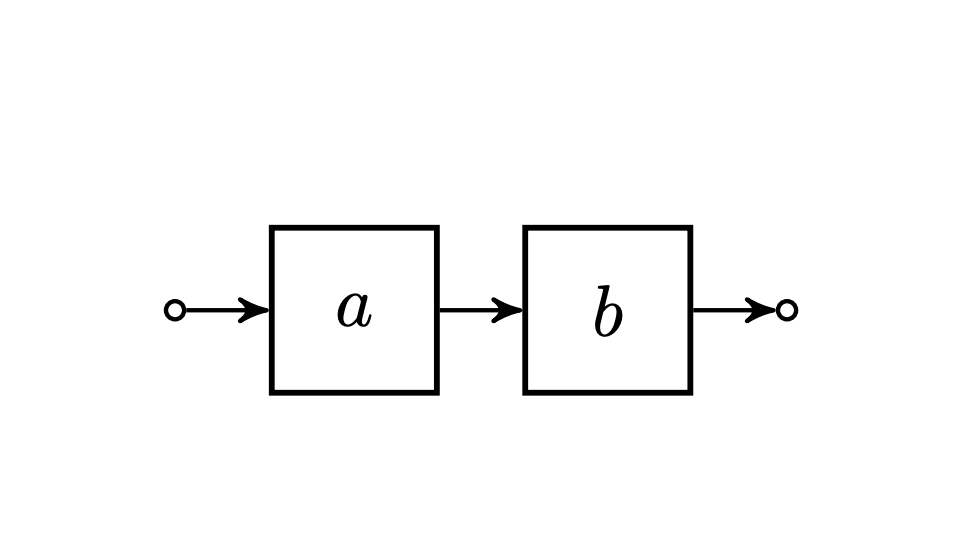
\includegraphics[width=0.5\linewidth]{img/automata_4}}
\caption{Умножение автоматов $ax$ и $bx$}
\label{img:automata:4}
\end{figure}

\noindent Данное кольцо, изоморфно кольцу $Q \cap \mathbb Z_p$, состоящему из рациональных чисел, знаменатели которых не делятся на $p$. В этом примере как элементы, так и операция сложения реализуется с помощью конечных автоматов, которые могут быть получены из единственного автомата $\Sigma_p$ при помощи операций суперпозиции и обратной связи. Для того чтобы в этом убедиться, достаточно показать, что любой автомат, реализующий функцию $f(x)=\frac{n}{m}x$, где $m, n \in \mathbb Z$ и $p$ не является делителем $m$, можно получить из $\Sigma_p$. Действительно, функция $f(x)=nx$, где $n \in \mathbb N$, реализуется при помощи суперпозиции из $n-1$ экземплярова автомата $\Sigma_p$, поскольку $nx=\underbrace{x+\cdots+x}_{n}$. Заметим, что автомат соответствующий функции $px$, является единичной задержкой, поскольку

$$ p(x_0+x_1p+\cdots)=x_0p+x_1+p^2+\cdots, $$

\noindent и сверхслово $x_0x_1\cdots$ переходит под его действием в сверхслово $0x_0x_1\cdots$. Из работы \cite{bib:automata:lunz} вытекает то, что мы уже умеем строить автоматы реализующие функции $ax$ и $bx$. Тогда, используя суперпозицию, построим функцию двух переменных $g(x,y)=ax+pby$ и, применив к ней операцию обратной связи по переменной $y$ (рис. \ref{img:automata:5}), получим функцию $h(x)=\frac{a}{1-pb}x$. Корректность построенной функции вытекает из уравнения $ax+pby=y$ и того факта, что $g(x,y)$ зависит от переменной $y$ с задержкой. Если взять $a=p-1$ и $b=1$, то $h(x)=-x$. 

\begin{figure}[H]
\centerline{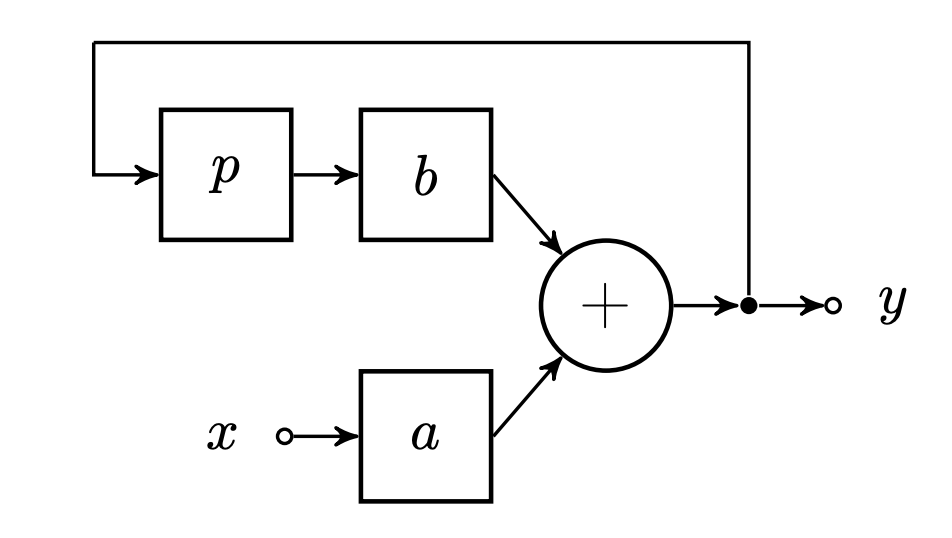
\includegraphics[width=0.5\linewidth]{img/automata_5}}
\caption{Автомат, реализующий функцию $h(x)=\frac{a}{1-pb}x$}
\label{img:automata:5}
\end{figure}

\noindent Тогда, используя суперпозицию, сможем выразить функцию $-nx=(-nx)$, где $n \in \mathbb N$, а так же константную функцию $0=x+(-x)$. Таким образом, мы можем реализовать любую функцию $ax$, где $a \in \mathbb Z$. Покажем, реализацию функции $\frac{1}{n}x$, где $n \in \mathbb N$ и $p$ не является делителем $n$. Поскольку числа $n$ и $p$ взаимно простые, всегда найдутся такие целые числа $a$ и $b$, что $na+pb=1$. Тогда, используя эти $a$ и $b$ в конструкции (рис. \ref{img:automata:5}, получим $h(x)=\frac{a}{1-pb}x=\frac{a}{na}=\frac{1}{n}x$. Заметим, что мы можем реализовать функцию $\frac{n}{m}x=n(\frac{1}{m}x)$ как суперпозицию функций. Таким образом, все функции вида $f(x)=cx$, где $c \in Q \cap \mathbb Z_p$, могут быть построены из $\Sigma_p$.

\subsection{Основные определения и обозначения}
Зафиксируем простое число $p$. Сопоставим каждому слову $\alpha=a(1)\cdots a(l)$ в алфавите $E_p=\{0,1,\cdots,p-1\}$ целое неотрицательное число $[\alpha]=a(1)+a(2)p+\cdots+a(l)p^{l-1}$. Договоримся, что пустому слову $\Lambda$ будет соответсвовать число $0$. Таким образом, слово $\alpha=a(1)a(2) \cdots a(l)$ является обращением записи $(a(1)a(2) \cdots a(l))_p$ числа $[\alpha]$ в $p$-ичной системе счисления \cite{bib:automata:tyapaev:2017,bib:automata:tyapaev:2018}.

\begin{defn} \cite{bib:automata:klapper}
Сверхсловом в алфавите $A$ называется проивзольная бесконечная последовательность $\alpha=a(1)a(2) \cdots$ элементов алфавита $A$. Сверхслова $\alpha=a(1)a(2) \cdots$ над алфавитом $E_p$ можно отождествлять с элементами $a(1)+a(2)p+\cdots$ множества $\mathbb Z_p$ целых $p$-адических чисел.
\end{defn}

\begin{defn} \cite{bib:automata:klapper}
Будем обозначать через $A|_l$ префикс $a(1)a(2)\ldots a(l)$ длины $l$, а через $a \downarrow_l$ соотвествующий бесконечных суффикс $a(l+1)a(l+2)\ldots a(l)$ сверхслова $\alpha$.
\end{defn}

\begin{defn}
$A^{\omega}$ - множество всех сверхслов над алфавитом $A$.	
\end{defn}

\begin{defn}
Функция $f: A^{\omega} \rightarrow B^{\omega}$ является детерминированной если для любых двух сверхслов $\alpha_1, \alpha_2 \in A^{\omega}$ и натурального $l$ из $\alpha_1|_l = \alpha_2|_l$ следует $f(\alpha_1)|_l = f(\alpha_2)|_l$.
\end{defn}

\begin{defn}
Для каждой детерминированной функции $f: A^{\omega} \rightarrow B^{\omega}$ и слова  $\alpha \in A^{*}$ введем функцию $f_{\alpha}(x) :=f(\alpha x)\downarrow_{\abs{\alpha}}$, которую будем называть остаточной функцией для $f$, соответствующую слову $\alpha$.	
\end{defn}


\begin{defn}
Детерминированную функцию $f: A^{\omega} \rightarrow B^{\omega}$, имеющую конечное число различных остаточных функций, назовем ограниченно"=детерминированной функцией.
\end{defn}


Известно\cite{bib:automata:aleshin}, что класс всех ограниченно-детерминированных функций совпадает с классом всех конечно-автоматных функций, реализуемых конечными инициальными детерминированными автоматами Мили. 


\begin{defn}
Детерминированную функцию $f: A^{\omega} \rightarrow B^{\omega}$ назовем обратимой, если она биективна, и, тем самым, для нее существует обратное отображение $f^{-1}: B^{\omega} \rightarrow A^{\omega}$, такое, что $f \circ f^{-1} = id_{A^\omega}$, $f \circ f^{-1}= id_{B^\omega}$. 
\end{defn}


Поскольку все остаточные функции $f_{\alpha}$ у обратимой функции $f$ так же обратимы, то у инициального автомата, реализующего $f$, в каждом состоянии $q$ функция выхода $\psi_q (x)=\psi(q,x)$ является биекций. В тоже время несложно показать, что любой обратимый автомат с таким свойством реализует обратимую ограниченно-детерминированную функцию. Для обратимой ограниченно-детерминированной функции $f$ функция $f^{-1}$ тоже является ограниченно-детерминированной функцией, причем с тем же весом, что и у $f$. Для того, чтобы в этом убедиться, достаточно рассмотреть диаграмму Мура автомата $\mathfrak{A}$ с начальным состоянием $q_0$, реализующего $f$ и каждую стрелку $q \xrightarrow{a/b} q^{'}$ в ней заменить на $q \xrightarrow{b/a} q^{'}$. Видно, что в результате получилась диаграмма некоторого нового автомата $\mathfrak{A}^{-1}$, и если в нем в качестве начального состояния выбрать опять $q_0$, то соответствующая ему ограниченно-детерминированная функция будет равна $f^{-1}$. В качестве примера можно посмотреть на рисунок \ref{img:automata:6}, где изображен обратимый автомат. Обратный к нему автомат показан на рисунке \ref{img:automata:7}. Он получается путем изменения $a/b$ на $b/a$ на всех его переходах.

\begin{figure}[H]
\centerline{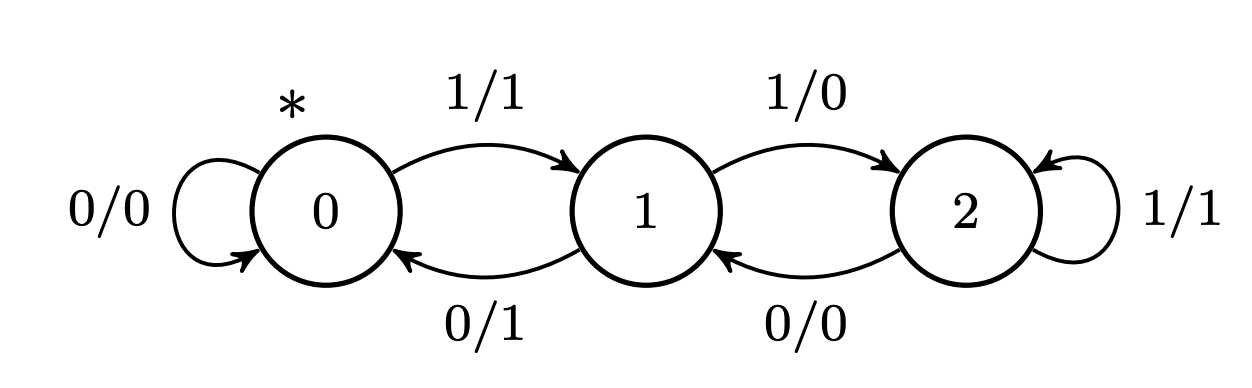
\includegraphics[width=0.5\linewidth]{img/automata_6}}
\caption{Диаграмма автомата $\mathfrak{A}_3$}
\label{img:automata:6}
\end{figure}

\begin{figure}[H]
\centerline{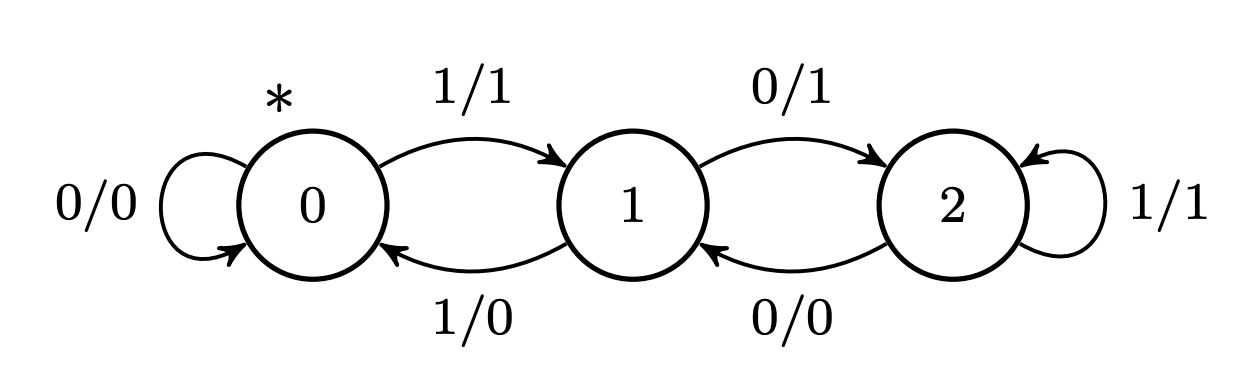
\includegraphics[width=0.5\linewidth]{img/automata_7}}
\caption{Диаграмма автомата $\mathfrak{A}_{\frac{1}{3}}$}
\label{img:automata:7}
\end{figure}


\subsection{Основная теорема о детерминированных функциях}
\begin{thethm}\cite{bib:crypto:anashin}
Детерминированная функция $f_\mathfrak{A}(s_0): \mathbb {Z}_p \rightarrow \mathbb {Z}_p$ соответствующая автомату $\mathfrak{A}(s_0)=\langle\mathbb {F}_p, \mathcal{S}, \mathbb {F}_p, S, O, s_0\rangle$, совместима, т.е. удовлетворяет $p$-адическому условию Липшица с константой $1$. Обратно, для каждой совместимой функции $f: \mathbb {Z}_p \rightarrow \mathbb {Z}_p$ существует автомат $\mathfrak{A}(s_0)=\langle\mathbb {F}_p, \mathcal{S}, \mathbb {F}_p, S, O, s_0\rangle$ такой, что $f=f_{\mathfrak{A}(s_0)}$.
\end{thethm}

\begin{proof}
Действительно, поскольку каждый $i$-й выходной символ $\psi_i = O(s_i, \chi_i)$ автомата зависит только от $i$-го состояния $s_i$ и от
$i$-го входного символа $\chi_i$, и поскольку состояние $s_i = S(s_{i-1}, \chi_{i-1})$ зависит только от $s_{i-1}$ и от $\chi_{i-1}$, и т.д. Таким образом, каждый выходной символ $\psi_i=\psi_i(\chi_0, \ldots, \chi_i) \in \mathbb F_p, i = 0,1,2,\ldots$, зависит только от входных символов $\chi_0, \ldots, \chi_i \in \mathbb F_p$ и не зависит от символов $\chi_{i+1}, \chi_{i+2}, \ldots$. Следовательно, детерминированная функция $f=f_\mathfrak{A}: \mathbb {Z}_p \rightarrow \mathbb {Z}_p$ имеет вид:

\begin{equation} \label{automata:1}
f: x = \sum_{i=0}^{\infty} \chi_{i}p^{i} \mapsto f(x) = \sum_{i=0}^{\infty}\psi_{i}(\chi_0,\ldots, \chi_i)p^i
\end{equation}

\noindent Другими словами, каждой детерминированной функции $f$ соответствует единственная последовательность отображений $\psi_i: \mathbb F^n_p\rightarrow \mathbb F_p$. Однако
каждая функция $f: \mathbb {Z}_p \rightarrow \mathbb {Z}_p$, имеющая вид \eqref{automata:1}, очевидно совместима, т.е. удовлетворяет $p$-адическому условию Липшица с константой $1$.

Обратно, пусть дана совместимая функция $f: \mathbb {Z}_p \rightarrow \mathbb {Z}_p$; тогда ее можно представить в виде \eqref{automata:1}. Построим автомат $\mathfrak{A}(s_0)=\langle\mathbb {F}_p, \mathcal{S}, \mathbb {F}_p, S, O, s_0\rangle$ такой что $f_\mathfrak{A}(s_0) = f$. Возьмем множество $\mathbb F_p^*$ всех непустых конечных слов над алфавитом $\mathbb F_p$, рассмотрим эти слова как представления натуральных чисел $\mathbb N = \{1, 2, 3, \ldots\}$ в системе счисления с основанием $p$
и перенумеруем слова в лексикографическом порядке в соответствии с
естественным порядком на $\mathbb N$. Таким образом мы установим взаимнооднозначное соответствие между всеми непустыми словами $w$ над алфавитом $\mathbb F_p$ и числами $i = 1, 2, 3, \ldots: w \leftrightarrow \nu(w), i \leftrightarrow \omega(i) (\nu(w) \in \mathbb N, \omega(i) \in \mathbb F_p^{*})$. Заметим, что $\nu(\omega(i)) = i, \omega(\nu(w)) = w$ для всех $i \in \mathbb N$ и всех непустых слов $w \in \mathbb F_p^{*}$. Будем считать, что $\omega(0)$ есть пустое слово.

В качестве множества $\mathcal{S}$ всех состояний автомата $\mathfrak{A}$ возьмем множество $\mathbb \mathbb N_{0} = \{0, 1, 2, 3, \ldots\}$, и возьмем $s_0 = 0$ в качестве начального состояния. Зададим функцию перехода $S$ следующим образом: $S(i, r) = \nu(r\omega(i))$, где $i = 0, 1, 2, \ldots r \in \mathbb F_p$; т.е. $S(i, r)$ равна номеру слова $r\omega(i)$, которое есть результат конкатенации слова $\omega(i)$ (с номером $i$) в качестве префикса (начала) с однобуквенным словом $r$ в качестве суффикса (окончания). Зададим функцию выхода следующим образом: $O(i, r) = \psi_{\abs{\omega(i)}}(r\omega(i))$, где символом $\abs{w}$ обозначается длина слова $w$ (длина пустого слова равна $0$). Отображение $\psi_i : F^{i+1}_p \rightarrow \mathbb F_p$ может рассматриваться как отображение множества всех слов длины $i + 1$ над алфавитом $\mathbb F_p$ во множество всех однобуквенных слов $\mathbb F_p, i = 0, 1, 2, \ldots$. Отметим, что при необходимости здесь и далее мы будем использовать без дополнительных оговорок естественное соответствие между словами длины $n$ и элементами кольца вычетов $m$ $\mathbb Z/p^n\mathbb Z$, также как и соответствие между множеством всех бесконечных слов $\mathbb F^\infty_p$ и кольцом $\mathbb Z_p$.

Поскольку $f$ удовлетворяет $p$-адическому условию Липшица с константой $1$, она непрерывна относительно $p$-адической метрики, а потому чтобы доказать, что $f=f_{\mathfrak{A}(s_0)}$ достаточно показать, что $f_{\mathfrak{A}(s_0)}(w) \equiv f(w)\pmod p^{\lambda(w)}$ для всех непустых слов $\omega \in \mathbb F_p^{*}$: действительно, если это так, то если дано бесконечное слово $w \in \mathbb F^\infty_p$, то последовательность $w \pmod {p^n}, n = 1, 2, 3, \ldots$, состоящая из конечных слов, сходится $p$-адически к $w$, т.е. $f(w) \pmod {p^n}$ сходится $p$-адически к $f(w)$ при $n$ стремящимся к бесконечности. 

Индукцией по $n$ докажем, что если входное слово $w$ имеет длину $n > 0$, то $f_{\mathfrak{A}(s_0)}(w) \equiv f(w) \pmod {p^n}$. Если $n = 1$, то $w \in \mathbb F_p$, и после того, как $w$ подано на вход, автомат $\mathfrak{A}$ перейдет в состояние $S(0, w) = \nu(w)$ и подаст на выход символ $O(0, w) = \psi_0(w) = f(w) \pmod p$, см. \eqref{automata:1}. 

Предположим, что утверждение верно для всех $n < k$ и докажем, что оно верно и при $n = k$. Рассмотрим слово $w$ длины $n$; тогда $w = rv$, где $r \in \mathbb F_p, \abs{v} = n-1$ (т.е. $w$ состоит из префикса $v$ и суффикса $r$). По предположению индукции, после того как слово $v$ будет подано на вход, автомат перейдет в состояние $\nu(v)$ и подаст на выход слово $v^{'} = f(v)\pmod {p^{n-1}}$. Следовательно, после того как на вход будет подан символ $r$, автомат подаст на выход символ $O(\nu(v), r) = \psi_{\abs{\omega(\nu(v))}}(r\omega(\nu(v)))=\psi_{\abs{v}}(rv)$. Стало быть, если подать на вход слово $w$, то автомат подаст на выход слово $v^{''} = (\psi_{\abs{v}}(rv))v^{'}$, которое есть результат конкатенации слова $v^{'} = f(v) \pmod {p^{n-1}}$ в качестве префикса с однобуквенным словом $\psi_{\abs{v}}(rv) \in \mathbb F_p$ в качестве суффикса. Однако $v^{''} = f(w) \pmod {p^n}$. \eqref{automata:1}. Этим завершается доказательство утверждения и теоремы.	
\end{proof}


\subsection{Построение автомата для функции вида $f(x)=cx$}
Для любого рационального числа $c=\frac{n}{m}$, где $n,m \in \mathbb Z$ и где $p$ не является делителем $m$, существует ограниченно-детерминированная функция $f: \mathbb Z_p \rightarrow \mathbb Z_p$ такая, что $f(x)=cx$. Обозначим через $\mathfrak{A}_c$ соотвествующий приведенный конечный автомат. Легко видеть, что для любой детерминированной функции $f: \mathbb Z_p \rightarrow \mathbb Z_p$ и слова $\alpha=a(1)a(2)\ldots a(l) \in E^l_p$ для соответствующей остаточной функции $f_\alpha (x)$ выполняется следующее соотношение:

\begin{equation} \label{automata:2}
f([\alpha]+p^lx)=[\beta]+p^l f_{\alpha}(x)
\end{equation}

\noindent где $\beta=b(1)b(2)\ldots b(l) =f(\alpha) \in E^l_p$:

\begin{equation} \label{automata:3}
\overbrace{\underbrace{a(1)\ldots a(l)}_{\alpha} \underbrace{x(1)x(2)\ldots}_{x}}^{[\alpha]+p^{l}x} \rightarrow
\boxed{f} \rightarrow \overbrace{\underbrace{b(1)\ldots b(l)}_{\beta} \underbrace{x(1)x(2)\ldots}_{x}}^{[\beta]+p^{l}f_{\alpha}(x)}
\end{equation}


\noindent Из соотношения \ref{automata:2} непосредственно следует формула для $f_{\alpha}(x)$:

\begin{equation} \label{automata:4}
f_{\alpha}(x)=\frac{f([\alpha]+p^{l}x)-[\beta]}{p^l}.
\end{equation}

\noindent Для начала опишем автомат $\mathfrak{A}_n$, где $n \in \mathbb N$. Применив формулу \ref{automata:4} к функции $f(x)=nx$, получим:

\begin{equation} \label{automata:5}
(nx)_{\alpha}=\frac{n([\alpha]+p^{l}x)-[\beta]}{p^l}	=nx+\frac{n[\alpha]-[\beta]}{p^l},
\end{equation}

\noindent где $[\beta]=n[\alpha] \pmod {p^l}$ (так как $f(\alpha)=\beta$). Следовательно, $n[\alpha]-[\beta]$ делится на $p^l$, и мы получаем более короткое представление:

\begin{equation} \label{automata:6}
(nx)_{\alpha}=nx+q,	
\end{equation}

\noindent где $q=\bigg[\frac{n[\alpha]}{p^l}\bigg] \in \{0, \ldots, n-1\}$, так как $n[\alpha]=p^l q+[\beta]$ и $[\alpha],[\beta] \in [0,p^l)$. Покажем, что $\forall q \in \{0, \ldots, n-1\} \quad \exists \alpha: \alpha \in E^l_p$, что  $q=\frac{n[\alpha]}{p^l}$.

\noindent Действительно, последнее эквивалентно следующему выражению:

\begin{equation} \label{automata:7}
p^l q \leq n[\alpha] \textless p^l q+ p^l.	
\end{equation}

\noindent Возьмем теперь достаточно больше $l$ так, чтобы выполнялось неравенство $p^l \textgreater n$, и положим $\alpha \in E^l_p$ равным $p$-ичной зависи числа $\bigg[\frac{p^l q}{n}\bigg]$, т.e. $[\alpha]=\bigg[\frac{p^l q}{n}\bigg]$. Тогда:

\begin{equation} \label{automata:8}
\frac{p^l q}{n} \leq [\alpha] \textless \frac{p^l q}{n} + 1 \Rightarrow p^l q \leq n[\alpha] \textless p^l q +n \Rightarrow p^l q \leq n[\alpha] \textless p^l q + p^l.
\end{equation}

\noindent Следовательно, слово $\alpha$ удовлетворяет условию (4) и $q=\bigg[\frac{n[\alpha]}{p^l}\bigg]$. Таким образом, показано что остаточные функции для $f(x)=nx$ полностью исчерпываются функциями $f^{(q)}(x)=nx+q$, где $q \in \{0, \ldots, n-1 \}$. Более того, все эти функции различны, поскольку $f^{(q)}(0) \neq f^{(q^{'})}(0)$ при $q \neq q^{'}$.

Такое наблюдение позволяет выбрать в качестве множества состояний приведенного автомата $\mathfrak{A}_n$, реализующего ограниченно-детерминированная функцию $nx$, множество $Q=\{0, \ldots, n-1 \}$. Опишем функцию переходов и функцию выходов автомата $\mathfrak{A}_n$. Применив формулу \ref{automata:4} к функции $f^{(q)}(x)=nx+q$ и однобуквенному слову $\alpha=a$, получим:


 \begin{equation} \label{automata:9}
 (nx+q)_{\alpha}=\frac{n(px+a)+q-b}{p}=nx+\frac{q+na-b}{p}	
 \end{equation}
 
\noindent где $b=na+q \pmod p$. Тогда $(nx+q)_\alpha = nx + q^{'}$, где $q^{'}=\frac{q+na-b}{p}$, и в автомате $\mathfrak{A}_n$ переход $q \xrightarrow{a/b} q^{'}$ существует тогда и только тогда, когда выполнено равенство:
 
 \begin{equation} \label{automata:10}
 	q+na=pq^{'}+b
 \end{equation}

\noindent Так как $q^{'} \in [0, n)$ и $b \in [0,p)$, то из равенства \ref{automata:10} следует, что

\begin{equation}
q^{'}=p^{-1}(q-a) \pmod n, \\
b=n^{-1}(a-q) \pmod p	
\end{equation}

\noindent где $p^{-1}$ - это обратный элемент для $p$ в кольце целых чисел по модулю $n$, а $n^{-1}$ - это обратный элемент для элемента $n$ в кольце целых чисел по модулю $p$. Оба элемента существуют, поскольку $n$ и $p$ - взаимно простые числа.

\conclusion
В данной курсовой работе был рассмотрен метод построения автомата для функции $f(x)=cx$, где $c=\frac{n}{m}, n,m \in \mathbb Z$. В дальнейшей научной работе планируется формализовать метод и расширить его для того, чтобы было возможно в виде автомата представлять любую полиномиальную функцию. 


\bibliographystyle{biblio/ugost}
\bibliography{biblio/biblio}

\end{document}